\documentclass{article}
\usepackage{ctex}
\usepackage{amssymb}
\usepackage{graphicx}
\usepackage[linesnumbered,ruled,vlined]{algorithm2e}
\usepackage{subfigure}
\usepackage[colorlinks,linkcolor=red]{hyperref}
\usepackage{float}
\usepackage{geometry}
\geometry{a4paper,scale=0.8}
\usepackage{algorithmicx}
\usepackage{arevmath}  % 数学符号
\usepackage[noend]{algpseudocode}
\usepackage{caption}
\usepackage{titlesec} 
\usepackage{enumerate}
\usepackage{blindtext}
\parindent=0pt

\usepackage{fancyhdr}
\pagestyle{fancy}
\fancyhf{}
\fancyhead[C]{密码学实验大作业}
\fancyfoot[C]{\thepage}
\renewcommand{\headrulewidth}{1.6pt} 
\setlength{\headwidth}{1.00\textwidth}
\titleformat{\section}{\LARGE\bfseries}{\thesection}{2em}{}
\geometry{a4paper,scale=0.8}
\title{\textbf{密码学实验大作业报告}}
\author{21371276 朱哲昊}
\date{2023年6月23日}
\begin{document}
	\begin{sloppypar}
	\maketitle\thispagestyle{fancy}
	\section{实验目的}
	设计一个封装完善、面向对象的密码库,包含各种常见的,可满足现代密码学基础功能的密码库,并有一定的差错检测功能。
	\section{实验环境}
	python 3.10
	\section{密码库内容}
	\subsection{基础数学库Math\_Crypto}

	\begin{enumerate}
		\item \textbf{扩展欧几里得算法}
		\item \textbf{最大公约数}
		\item \textbf{求逆元}
		\item \textbf{素数检测} 采用Miller Rabin素性检测
		\item \textbf{生成大素数} 输入需要生成素数的二进制位数要求
		\item \textbf{快速模幂运算} 
	\end{enumerate}
	\subsection{SM2签名函数}
	\begin{enumerate}
		\item \textbf{sign签名函数}
		Python类中的一个方法,名为sign。它接受五个参数:ID\_A,P\_A,M,d\_A和k。它首先调用类中的另一个方法get\_Z\_A来获取Z\_A值,然后将Z\_A和M编码后的十六进制字符串拼接起来,使用SM3算法计算哈希值e。接下来,它使用椭圆曲线加密算法计算出$(x1, y1)$,然后使用$r = (e + x1) \% n$计算出$r$,再使用$s = (invmod(1 + d_A, n) * (k - r * d_A)) \% n$计算出$s$。最后,它返回$r$和$s$。
		\item \textbf{verify验签函数}
		Python函数,名为verify,接受五个参数:ID\_A,P\_A,M,r和s。函数中使用了SM3哈希算法,对M进行哈希,并将结果与Z\_A拼接后再进行哈希,得到e。接着,计算t、x1、y1、x2、y2、x和y,并计算R。最后,判断R是否等于r,如果是则返回True,否则返回False。
	\end{enumerate}
	\subsection{SM3杂凑函数}
	\begin{enumerate}
		\item \textbf{sm3\_hash函数}
		生成sm3的杂凑值,SM3哈希函数的实现。它将输入的消息进行填充,然后使用迭代压缩算法进行哈希计算。其中,T是一个常量数组,Mlen表示消息的长度,temp是计算出的哈希值。
		
		
	\end{enumerate}
	\subsection{SM4分组密码实现}
	SM4(原名SMS4)是中华人民共和国政府采用的一种分组密码标准,由国家密码管理局于2012年3月21日发布,在商用密码体系中,SM4主要用于数据加密,其算法公开,分组长度与密钥长度均为128bit,加密算法与密钥扩展算法都采用32轮非线性迭代结构,S盒为固定的8比特输入8比特输出。输入为一个128位的整数x,输出也是一个128位的整数。首先将x拆分成4个32位的整数,然后进行32轮迭代,每轮迭代都会进行一系列的操作,包括异或、S盒替换、线性变换等,最后得到加密或解密后的结果。具体的实现细节可以参考代码中的注释。
	\begin{enumerate}
		\item \textbf{CTR模式}
		SM4算法的CTR模式实现,用于文件的加密和解密。其中,file\_path是文件路径,IV是初始化向量,MODE为1表示加密,0表示解密。代码中使用了一个CTR\_get\_key函数来生成密钥,然后对文件进行分块加密或解密。加密后的文件名为file\_name.SM4\_CTR。
		\item \textbf{CFB模式}
		这段代码是一个SM4算法的实现,用于对文件进行加密和解密。它接受文件路径、初始向量、字节数和模式作为输入,输出加密或解密后的文件。在加密模式下,它将读取文件并将其分成n个字节的块,然后使用CFB模式对每个块进行加密。在解密模式下,它将读取加密后的文件并使用CFB模式对每个块进行解密。
		
		
	\end{enumerate}
	\subsection{RSA公钥密码体制}
	\begin{enumerate}
		\item \textbf{RSA encryption/decryption}
		这是一个Python类中的两个方法,用于加密和解密数据。其中,encrypt方法接受一个参数m,使用类中的e\_or\_d和n属性对m进行加密,并返回加密后的结果。而decrypt方法接受一个参数c,使用类中的e\_or\_d和n属性对c进行解密,并返回解密后的结果。fastpower函数可能是一个用于快速幂运算的函数。
		
		\item \textbf{RSA keygenerate}
		 RSA加密算法的密钥生成函数。第一个函数根据给定的两个质数p和q生成公钥(e,n),其中e是一个与(p-1)(q-1)互质的随机质数,d是e的模(p-1)(q-1)的逆元。第二个函数根据给定的位数N生成公钥(e,n),其中p和q是N位的大质数。在两个函数中,都使用了一个invmod函数来计算模逆元。
		
		\item \textbf{RSA OAEP}
		 RSA算法的加密函数,使用OAEP填充方式。其中k表示RSA算法的安全参数,m表示明文,L表示标签,seed表示随机数。函数会先进行长度检查,然后使用EME\_OAEP函数进行填充,最后进行加密并返回密文。
		
		​ RSA加密算法中的OAEP解密函数。它接受三个参数:k表示密钥长度,c表示密文,L表示标签。函数首先计算出L的长度,然后根据密钥长度和标签长度检查密文长度是否合法。接着将密文转换为整数C,并检查C是否小于n。然后使用私钥解密C得到明文m,并将m转换为十六进制字符串EM。接着检查EM的长度是否合法,如果不合法则抛出异常。然后将EM填充到长度为2k的字符串中,并使用EME-OAEP解码算法解码得到明文M。最后将M转换为十六进制字符串并返回。
	\end{enumerate}
	\section{差错检测}
	对各个输入进行检测,以及在运算过程中进行检测,检测到错误时抛出对应的错误样式,达到对使用者便利的目的。例如RSA的输入检测:
	\begin{figure}[H]
		\centering
		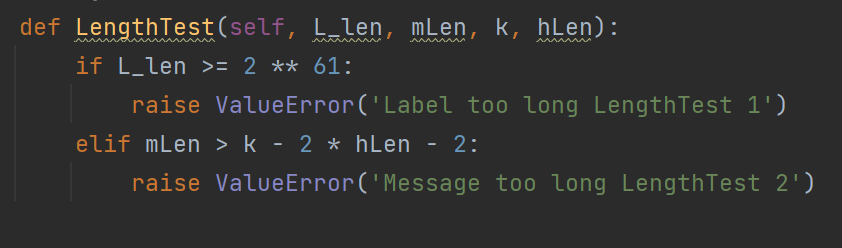
\includegraphics[scale=0.9]{pic/rsa length test.png}
		\caption{rsa input test}
		\label{figure}
		
	\end{figure}

	再比如,RSA OAEP的时候encode的编码检测
	\begin{figure}[H]
		\centering
		\includegraphics[scale=0.8]{pic/RSA OAEP encoding error.png}
		\caption{rsa oaep encoding error test}
		\label{figure}
		
	\end{figure}
	
	\section{测试结果}
	\href{run:../test result -.html}{python test.py测试结果}
	
	显示12个测试函数都通过了测试。各个测试数据均选用密码学实验课中的实验测试数据,证明了本密码库的功能完整,程序编写正确,能实现密码库的需求,是一个合格的密码库。
	\section{使用说明}
	详细的使用说明参见\href{../user's Guide.pdf}{user's Guide} 或者 markdown形式文件\href{../user's Guide.md}{user's Guide}
	\section{实验心得}
	集成之前的密码算法到密码库的工作量比想象大好多,要对密码算法重新调整输入输出以及各种参数,还要对部分算法支持文件输入输出。密码库封装好之后可以直接调用,以后如果要用得到的话会方便很多。
	
\end{sloppypar}
\end{document}
